\documentclass[titlepage]{article}
\usepackage[utf8]{inputenc}
\usepackage{geometry}
\geometry{a4paper, margin=1in}
 \usepackage[draft]{graphicx} %uncomment this for faster compiles.
%\usepackage{graphicx}  %uncomment this for pictures to load in.
\usepackage{float}
\usepackage{subcaption}
\usepackage{listings}
\usepackage{caption}
\usepackage[table]{xcolor} % Enable coloring of table cells
\usepackage{booktabs} % For formal tables
\usepackage{array}
\definecolor{lightgray}{gray}{0.9}

\begin{document}


\title{Software Design Document\\ \textbf{Insight Glass}}
\author{Aser Osama - 202101266 \\ Aya Sherif - 202100642 \\ Gehan Sherif - 201902069 \\ Omar Ayman 202100443 }
\date{Version 1.0 \\\ \today}


\maketitle
\tableofcontents


\newpage

\section{Project Overview}
\subsection{Project idea}
Our project's main goal is to help professionals from different disciplines start their careers at companies where 
they can thrive. This will be achieved through radical transparency of the companies, breaking down all barriers 
and problems in the Egyptian job markets that lead to discrimination, pay gaps, and toxic work environments.

\subsection{Vision}
The vision is to transform the Egyptian job market by empowering individuals to make informed decisions about their 
career path. The project aims to address common issues of job seekers struggling to identify suitable employment 
opportunities and being locked into unfavorable work environments due to contractual obligations. By providing 
comprehensive insight into the company and facilitating transparent communication between job seekers and 
employers, the project seeks to create a dynamic ecosystem that fosters mutual growth, and they are satisfied 

\subsection{Competitive Analysis}
In Egypt's job market, traditional methods of hiring still dominate, with a reliance on personal connections and 
in-person applications. However, the emergence of online platforms has introduced new avenues for job 
seekers. Two prominent competitors in this space are Glassdoor.

\subsubsection*{Glassdoor}
Glassdoor, our main competitor, is a well-established platform known for providing company reviews, salary information, and job 
listings. While it offers valuable insights into company cultures and employee experiences globally, its 
adaptation to the Egyptian context might be limited. Glassdoor primarily relies on user-generated content, 
which may vary in quantity and quality, especially for companies with a smaller presence in Egypt. 
Additionally, the platform's focus on larger corporations might overlook opportunities within smaller or niche 
companies in the Egyptian job market.

\newpage

\section{System Technical Overview}
\subsection{System Architecture}
We will use a simple, reliable, yet scalable architecture. We will use a Frontend and API connecting to a 
backend model. It is a simple model, however, it will be comfortably scalable using Kubernetes, Azure, or any 
other load balancers as we expand to have more people using our service. We will use virtualization in
expandability and have spare servers be there in case of breakdowns to minimize downtime. 

\begin{figure}[H]
    \centering
    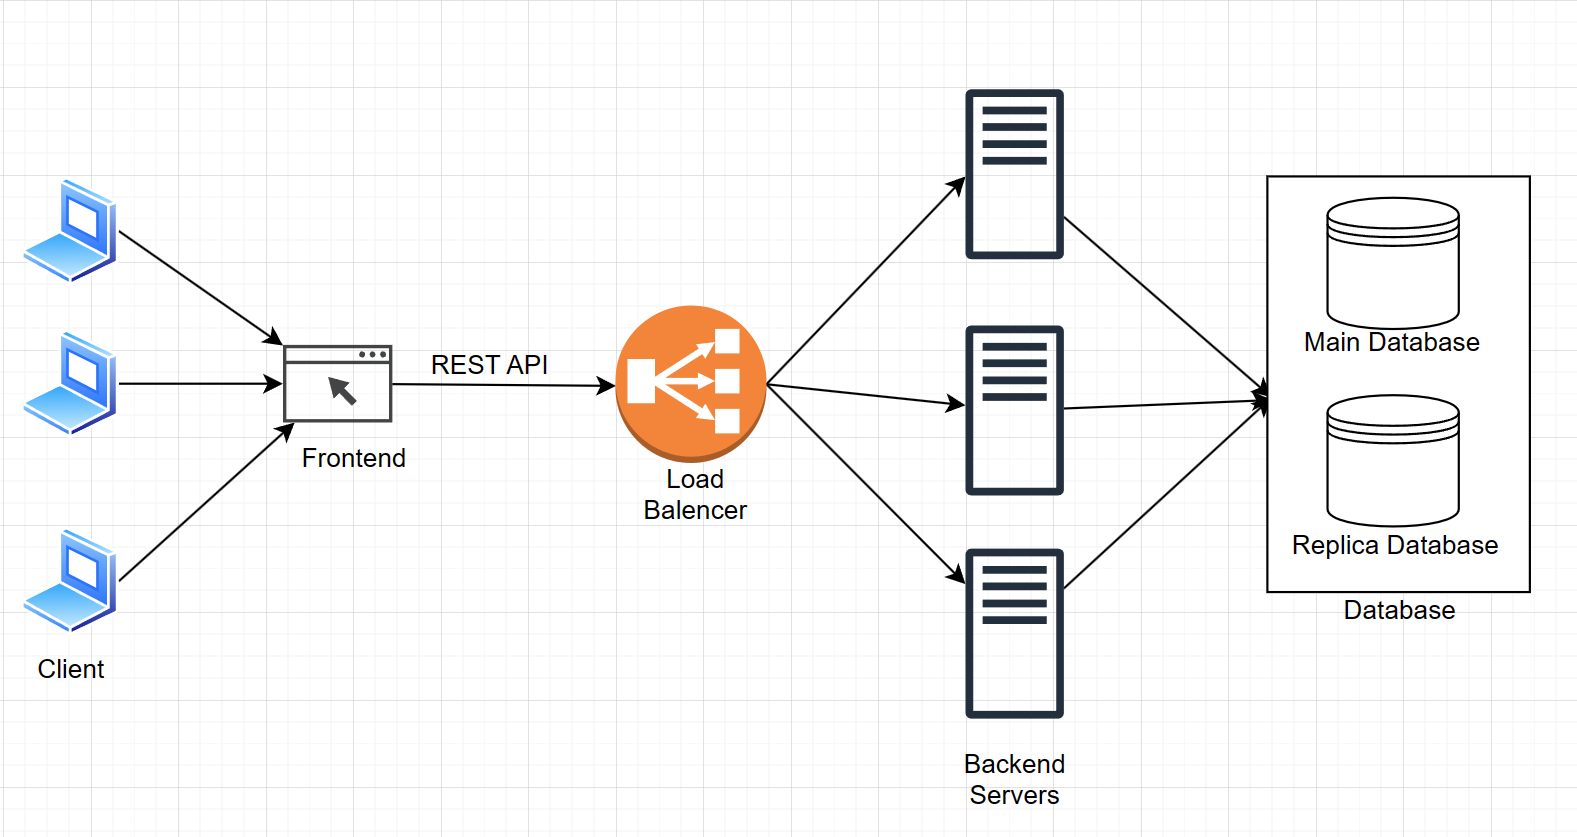
\includegraphics[width=0.8\textwidth]{Images/ArchOverview.png}
    \caption{System Architecture Overview}
\end{figure}

\subsection{Used Technologies}
\begin{itemize}
    \item \textbf{Frontend:} React.js for building a responsive and dynamic user interface
    \item \textbf{Backend:} ASP.NET Web API in .NET 8 for server-side logic, providing a reliable and efficient foundation.
    \item \textbf{Database:} MySQL/MariaDB for storing user data, reviews, and job listings, chosen for its flexibility with 
    schema design and easy to find support. Interaction with the database will be through the Entity Framework 
    Core ORM
    \item \textbf{Authentication:} Identity framework with cookie-based authentication will be used.
\end{itemize}

\newpage

\section{Biggest Challenges and Mitigations}
\subsection{Challenges}
Egypt is currently very behind in terms of modernizing the hiring process, therefore it would be incredibly 
difficult to try and convince companies and people to change their old ways. Adoption of the application will 
also be difficult due to the reason we would most likely function as a startup which is also not looked to highly 
of in Egypt. Aside from initial adoption of the application, building a community of verified employees to 
provide us with reviews and insight might be also difficult as people tend to not be as open with salaries or job 
experience here. We will be challenging a lot of old stereotypes and set in stone rules of the workplace with our 
application. A more technical issue we might face are fake reviews. Finally, the legalities of sharing job reviews 
and such are not too certain in Egypt so it could be risky if not dealt with correctly.

\subsection{Solutions}
The technical issue of fake reviews could be easily solved by adding multiple human verification stages to our 
website as well as requiring identification and proof of employment to be able to post reviews that would affect 
the overall company rating while also keeping a section for unverified reviews. As for the adoption issues,
however, we could attempt to gain the user’s trust by getting affiliation with trusted companies or businesses 
figures. However, it is most likely that the issue would simple be resolved with time and we have no real choice 
to kickstart our popularity. Finally, for the legalities, we could employee a part time or on demand legal team to 
help us sort it out.

\section{Feasibility Matrix}

%colorless table:
% \begin{table}[h]
% \centering
% \caption{Feasibility Assessment}
% \label{tab:feasibility_assessment}
% \begin{tabular}{@{}lp{5cm}ccc@{}}
% \toprule
% Criteria             & Description                                                                                        & Score & Weight & Total Score \\ \midrule
% Technical Feasibility & The project's technical requirements include platform development and data gathering processes.     & 4     & 25     & 100        \\
% Economic Feasibility  & The financial viability of the project, including initial investment, operating costs, and revenue generation. & 3     & 20     & 60         \\
% Legal Feasibility     & Compliance with legal regulations and potential risks related to data privacy, intellectual property, etc.        & 4     & 20     & 80         \\
% Operational Feasibility & The project's practical implementation and operational processes, including user engagement and support.  & 5     & 35     & 175        \\ \bottomrule
% \end{tabular}
% \end{table}

\begin{table}[h]
    \centering
    \caption{Feasibility Assessment}
    \label{table:feasibility}
    \begin{tabular}{>{\raggedright}m{3.5cm} >{\raggedright\arraybackslash}m{5.5cm} c c c}
    \toprule
    \textbf{Criteria} & \textbf{Description} & \textbf{Score} & \textbf{Weight} & \textbf{Total Score} \\ 
    \midrule
    \rowcolor{lightgray} Technical Feasibility & The project's technical requirements include platform development and data gathering processes. & 4 & 25 & 100 \\
    Economic Feasibility & The financial viability of the project, including initial investment, operating costs, and revenue generation. & 3 & 20 & 60 \\
    \rowcolor{lightgray} Legal Feasibility & Compliance with legal regulations and potential risks related to data privacy, intellectual property, etc. & 4 & 20 & 80 \\
    Operational Feasibility & The project's practical implementation and operational processes, including user engagement and support. & 5 & 35 & 175 \\
    \bottomrule
    \end{tabular}
    \end{table}


\section{Interface Design}
\subsection{External Interfaces}
Detail the design of external interface connections, protocols, and standards.

\subsection{User Interfaces}
Describe the design of the user interface, including screen layouts and user interaction flows.

\section{Dynamic System Design}
Explain the dynamic processes, activities, and tasks within the system, including any state diagrams or sequence diagrams.

\section{Functional Requirements}
\subsection{User Registration and Authentication}
Users can sign up using email or social media accounts and verify their identity through email or phone number. Passwords should be securely stored and encrypted.
\subsection{Profile Management}
Users can manage their profiles, edit personal information, upload resumes, set privacy preferences, and track their activity history (e.g., jobs applied to, reviews submitted).
\subsection{Comprehensive Company Profiles:}
The platform should feature detailed company profiles, including employee reviews, work culture assessments, salary information, and benefits offered.

\subsection{Advanced Job Search Filters:}
Users should be able to search for jobs using advanced filters tailored to the Egyptian job market, including location, industry, salary range, employment type, and company rating.

\subsection{Direct Communication Channels:}
The platform should facilitate direct communication between job seekers and companies, allowing inquiries about job openings, company culture, and application processes.

\subsection{Transparent Job Listings:}
Job listings should provide transparent information about job requirements, responsibilities, compensation packages, and company details to help job seekers make informed decisions.

\subsection{User-Driven Community Features:}
Users should have the ability to request the inclusion of companies not listed on the platform and contribute to the community by sharing insights and experiences.

\subsection{Risk Mitigation Mechanisms:}
The platform should implement mechanisms to vet companies before listing them, address concerns such as contractual obligations, and provide channels for users to report unfavorable experiences.

\subsection{Review Submission}
Users can submit reviews for companies they have worked for, rating aspects such as work culture, management, salary and benefits, and career growth opportunities. Reviews should be moderated to ensure authenticity and professionalism.

\subsection{Interactive Discussion Forums:}
The platform should host interactive discussion forums and groups focused on career development, industry insights, and job search strategies, encouraging user engagement and knowledge-sharing.

\subsection{Localized Content and Language Support:}
The platform should offer localized content and language support tailored to the Egyptian market, ensuring a user-friendly experience for both job seekers and employers.

\subsection{Integration with Social Media Platforms:}
Users should have the option to integrate their social media profiles with the platform for seamless networking and profile completion, enhancing their visibility to potential employers.


\subsection{Salary Benchmarking Tools:}
The platform should provide salary benchmarking tools based on industry standards and user-reported data, helping job seekers evaluate compensation packages and negotiate effectively.

\subsection{Interview Preparation Resources:}
Users can share and access interview experiences specific to the Egyptian job market, including insights on common interview questions, cultural expectations, and company-specific practices.


\subsection{Feedback and Ratings System:}
The platform should include a feedback and ratings system for companies, allowing users to rate their experiences and provide constructive feedback to improve employer practices.

\subsection{Data Privacy and Security Measures:}
The platform should implement robust data privacy and security measures to protect user information and comply with Egyptian data protection regulations.

\subsection{Analytics and Insights Dashboard:}
Administrators should have access to an analytics and insights dashboard to track user engagement, job market trends, and platform performance metrics.

\subsection{Collaboration with Educational Institutions:}
The platform should collaborate with educational institutions to provide career guidance, internship opportunities, and job placement services for students and recent graduates.

\subsection{Promotion of Diversity and Inclusion:}
The platform should actively promote diversity and inclusion in the workplace by featuring companies with inclusive policies and initiatives and encouraging equal opportunities for all job seekers.

\subsection{Continuous Improvement and Updates:}
The platform should undergo continuous improvement and updates based on user feedback, technological advancements, and changes in the job market landscape to enhance user experience and platform functionality.

\section{Non-Functional Requirements}
\subsection{Performance and Scalability}

The platform   should be highly responsive, with fast loading times and smooth navigation, ensuring a seamless user experience for job seekers and employers accessing the platform from various devices and locations across Egypt.
The system architecture should be scalable to accommodate growing user traffic and data volume, allowing the platform to handle increased user activity and maintain performance reliability during peak usage periods.
\subsection{Data Privacy and Security Compliance}

The platform should adhere to strict data privacy and security standards, ensuring the confidentiality, integrity, and availability of user data.
Compliance measures should align with Egyptian data protection regulations, such as the Data Protection Law, ensuring that user information is stored, processed, and transmitted securely to mitigate the risk of unauthorized access, data breaches, and privacy violations.
\appendix
\section{Appendix A: Glossary}
\section{Appendix B: Feasibility Study}
\section{Appendix C: Issue Log}

\end{document}
